\chapter{The k-Means Clustering Algorithms}\label{chapter:kmeans}

\section{Motivation}

In this work, the data mining algorithm k-Means will be implemented in HyPer using the operator model, in order to show a proof-of-concept implementation.
\\
K-means is a well-studied clustering algorithms, partitioning a data set into k clusters, where all data objects within a cluster are similar to each other, and dissimilar to the data objects in the other cluster. The goal is to find the best clustering, minimizing the total squared distance between each data point and its assigned center. While the solution to that problem is NP-hard, there are several heuristics, in particular the Lloyed algorithm, which is a local search solution to this problem. 
\\
The algorithm is one of the most popular data mining algorithms. In fact, a survey of clustering data mining techniques in 2002 states that the algoritm “is by far the most popular clustering algorithm used in scientific and industrial applications”. K-means is also part of the 10 top data mining algorithms identified by the IEEE International Conference on Data Mining (ICDM) in December 2006, next to other famous algorithms such as SVM and PageRank. 

\section{The Lloyd Algorithms}

In the following paragraph we explain the Lloyed algorithm, usually referred as k-Means in literature and in this work as well. The algorithm starts with k arbitrary center points, typically chosen at random from the data points. Then, each data point is assigned to the closest center, using a distance function. Usually, the euclidean distance is used, other implementations allow to choose between several distance functions. After assigning each data point to its closest center, the centers gets updated, i.e. the center is the mean coordinate of all the data points assigned to this center. Then the process begins again, assigning the data points again, now to the updated centers. This continues until the process stabilizes and the algorithm converges.
\\
Formally, the k-Means problem and the k-Means algorithm are described the following: For a given integer k and a data set of n data points X Teilmenge of Rd, choose k Centers c to minimize the sum of squared error function,
\begin{equation*}
sse = \Sigma_{x \in X} min_{c \in C} ||x - c||^2
\end{equation*}
When found the centers, we know which data points belongs to the same center and we have found our clustering.
\\
The k-Means algorithms is described then the follwing:

\begin{enumerate} 
\item Arbitrarily choose $k$ centers $C = \{c_1, c_2, \cdots, c_k\}$ uniformly at random from $X$.
\item For each $i \in \{1, \cdots, k\}$, set the cluster $C_i$ to be the set of points in $X$ that are closer to cluster $c_i$ than to any other cluster $c_j$ for all $j \neq i$.
\item For each $i \in \{1, \cdots, k\}$, set $c_i$ as the center of all points assigned to $C_i$: 

\begin{equation*}
c_i = \frac{1}{|C_i|} \Sigma_{x \in C_i} x.
\end{equation*}

\item Repeat Steps 2 and 3 until $C$ no longer changes, i.e. the algorithm converges.
\end{enumerate}


\section{Example}

$x_0(3,9), x_1(2,5), x_2(5,8), x_3(7,5), x_4(4,2)$

Initial center of the Clusters: $c_0(3,9), c_1(4,2)$

\begin{table}[htsb]
  \caption[Computations in Iterations 1]{Computations in Iterations 1.}\label{tab:kmeans_iter_1}
  \centering
  \begin{tabular}{l l l l}
    \toprule
      Distance & $c_0(3,9)$ & $c_1(4,2)$ & Cluster \\
    \midrule
        $x_0(3,9)$ & 0.00 & 7.07 & $C_0$ \\
        $x_1(2,5)$ & 4.12 & 3.61 & $C_1$ \\
        $x_2(5,8)$ & 2.24 & 6.08 & $C_0$ \\
        $x_3(7,5)$ & 5.66 & 4.24 & $C_1$ \\
        $x_4(4,2)$ & 7.07 & 0.00 & $C_1$ \\
    \bottomrule
  \end{tabular}
\end{table}


\begin{table}[htsb]
  \caption[Computations in Iterations 2]{Computations in Iterations 2.}\label{tab:kmeans_iter_1}
  \centering
  \begin{tabular}{l l l l}
    \toprule
      Distance & $c_0(4,8.5)$ & $c_1(4.33,4)$ & Cluster \\
    \midrule
        $x_0(3,9)$ & 1.12 & 5.17 & $C_0$ \\
        $x_1(2,5)$ & 4.03 & 2.54 & $C_1$ \\
        $x_2(5,8)$ & 1.12 & 4.06 & $C_0$ \\
        $x_3(7,5)$ & 4.61 & 2.85 & $C_1$ \\
        $x_4(4,2)$ & 6.50 & 2.02 & $C_1$ \\
    \bottomrule
  \end{tabular}
\end{table}


\begin{figure}[htsb]
  \centering
  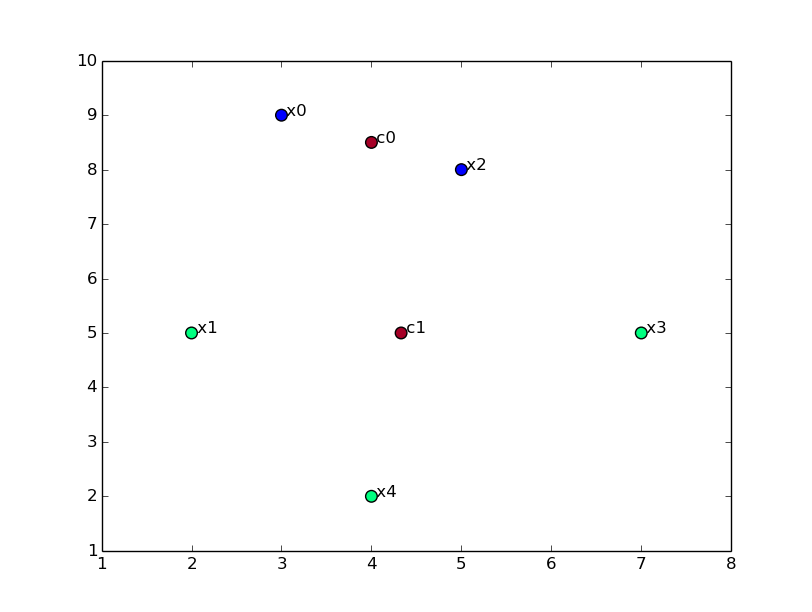
\includegraphics[scale=0.5, trim="0cm 1cm 0cm 0cm"]{figures/kmeans_example}
  \caption[k-Means Example Clustering]{k-Means Example Clustering.}\label{fig:kmeans_example}
\end{figure}




\section{The k-Means++ Initialization Strategy}

This simple algorithm terminates in practice very fast and provides mostly good result, even though the clustering can be arbitrarily bad for some data sets. Particularly, the random choosing of the initial cluster centers can lead to a bad clustering, which cannot be changed during the clustering process. Therefore,  propose a variation to the k-Means initialization strategy, called k-means++. The centers are still chosen randomly from the data points, but the ata points are weighted according to their distance from the closest center already chosen. Therefore, the probability that of choosing data points as center that are far away get higher, leading to improvements, both in speed and accuracy of the clustering.
\\
Formally, k-means++ can be described the following:
Let D(x) the shortest distance from a data point the closest, already picked center. 

\begin{enumerate} 
\item Take the first center $c1$, chosen uniformly at random from $X$.
\item The next center $c_i$ is choosen from $x \in X$ with the propability 

\begin{equation*}
\frac {D(x)^2} {\Sigma_{x \in X} D(x)^2}.
\end{equation*}

\item Repeat Step 2 until all $k$ centers are selected.
\item Continue as in the standard k-Means algorithm.
\end{enumerate}

Most clustering tools implement a k-means++ initialization strategy for k-means, therefore we will also test k-means++ on HyPer.
\\
Since the algorithm is very popular and easy to understand, makes it suitable for the first implementation of a data mining algorithm on HyPer. All data mining tools we looked at (see related work) are implementing k-Means, which makes it neat to compare regarding the running time. The cluster compactness, i.e. the sum of squared errors is a good quality measurement of the clustering, and allows very good comparability. Since the algorithm is well-defined, we can expect that the data mining tools are implementing the actual k-Means algorithms, only adapting to their programming model. Another nice fact is that many data mining tools also implement k-Means++ as initialization strategy, another thing that can be compared.
Parts of K-means can be executed in parallel, and since HyPer supports parallel computation, it will be another interesting research to evaluate how single-threaded execution of K-means vs a multi-threaded computation. We are expecting tremendous performance gains executing HyPer on a multicore machine, and it will be interesting to compare these results to the results of big data computing, such as MapReduce or Apache 


